

Díky tomu, že si přesně určíme, kdo je cílový uživatel naší aplikace, a k tomu dáme do hromady, co uživatel od naší aplikace očekává.
Jsme tedy nyní schopni bez větších problémů teoreticky navrhnout architekturu našeho systému a přesně popsat požadovanou funkcionalitu, jakou budou disponovat jeho jednotlivé části.
Tato sekce se bude zabývat analýzou a návrhem architektury systému Coopmaster dle požadavků ze sekce~\ref{ch:tvorba-zadani}.

\section{Šlužby dle jednotlivých potřeb uživatele}\label{sec:microservices}
Jako teoretický model na základě kterého, budeme organizovat a třídit funkcionalitu, jsem zvolil mikroservisní architekturu(sekce~\ref{sec:microservice-architecture}).
Tento způsob rozvržení zodpovědnosti částí systému jsem zvolil, díky velké možnosti rozšíření, zapouzdření funkcionality a snadné úpravě jednotlivých služeb bez nutnosti kompletního restartu systému případně znovunasazení.\newline
Jako programovací jazyk pro tvorbu služeb je zvolen programovací jazyk Python(sekce~\ref{sec:python}).
Python byl vybrán kvůli jeho univerzálnosti, snadné syntaxi a podpoře ze strany vývojářů a komunity.\newline
Pro realizaci, konfiguraci a síťování mikroservistní architektury je použit Docker Engine(sekce~\ref{sec:kontejnerizace}) společně s rozšířením Docker Compose.\newline
Na základě předchozích rozhodnutí jsem tedy systém rozdělil do jednotlivých mikroslužeb, tak aby vznikla robustní a rozšiřitelná mikroservisní architektura a byly splněny všechyn uživatelské požadavky, které jsme si určili (\ref{ch:tvorba-zadani}).\newline
Bylo tedy navrženo 8 služeb, které obsahují námi naprogramovanou funkcionalitu a dohromady společně s hardwarovými prvky tvoří systém Coopmaster.
\begin{itemize}
    \item Camera driver (\ref{sec:camera-driver})
    \item Scale driver (\ref{sec:scale-driver})
    \item Room driver (\ref{sec:room-driver})
    \item Health checker (\ref{sec:health-checker})
    \item Room assistant (\ref{sec:room-assistant})
    \item Nest watcher (\ref{sec:nest-watcher})
    \item Dog alarm (\ref{sec:dog-alarm})
    \item Chicken watch guard (\ref{sec:chicken-watch-guard})
\end{itemize}

\section{Systému pro uživatelské rozhraní a automatizaci}\label{sec:systemu-pro-uzivatelske-rozhrani-a-automatizaci}
Podstatnou otázkou bylo, zda se pouštět do tvorby kompletně vlastního systému pro uživatelského rozhraní a automatizaci.
Po zvážení časové náročnosti, technologické náročnosti a komplexnosti takového systému, mi bylo jasné, že tudy cesta nepovede.
Bylo tedy třeba najít open source systém, který již touto funkcionalitou disponuje.
Nakonec jsem zvolil systém Home Assistant, protože jsem s ním již dříve pracoval a mám s ním dobré zkušenosti.
Home Assistant má na internetu také rozsáhlou podporu a komunitu s množstvým nápadů a již hotových řešení pro inspiraci.
Popis toho, jak je nakonfigurováno uživatelské rozhraní v Home Assistantovi, je popsáno v sekci~\ref{sec:tvorba-gui-rozhrani}.

\section{Komunikace mezi Backendem a Frontendem}\label{sec:komunikace-mezi-backendem-a-frontendem}
Je třeba zajistit komunikaci mezi Home Assistantem a Coopmaster službami.
Tuto úlohu musíme přijmout velice zodpovědně a navrhnout řešení, které půjde opět snadno rozšířit a modifikovat.
Nelze proto použít klasické HTTP(sekce~\ref{sec:http-rest}), z toho důvodu že bychom komunikaci vázali na buď doménové jméno a port nebo ip adresu a port.
Toto řešení má problém v tom, že pokud bychom potřebovali změnit, buď umístění částí služeb nebo port jedné ze služeb, bylo by třeba překonfigurovat i home assistanta.
Dalším problém nastane, když potřebujeme z některé ze služeb poslat například notifikaci do Home Assistanta, je pro to potřeba, aby jednotlivé služby věděli, kde na síti Home Assistant běží, což je věc, která se může měnit, a museli bychom naopak přenastavovat jednotlivé služby.
Jako řešení se nabízí použít messaging konkrétně třeba technologii MQTT(sekce~\ref{sec:mqtt}).
Tato technologie se běžně používá u IoT zařízení a pro naše použití je vynikajícím řešením.

\section{Hardwarová zařízení}\label{sec:hardwarova-zarizeni}
Tuto sekci je velmi důležité dobře a správně navrhnout, protože náš systém bude pracovat s daty z reálného světa.
Tato data musejí získávat k tomu určená zařízení a na jejich přesnosti závisý efektivita a správnost chování zbytku systému.
Musíme tedy navrhnout a realizovat několik zařízení, která společně budou plnit následující úlohy
\begin{itemize}
    \item snímání stavů hnízd
    \item ovládatní dvířek
    \item snímání teploty a vlhkosti
    \item snímání scén v kurníku a ve výběhu
\end{itemize}

\subsection{Snímání stavů hnízd}
Všechny případy, které potřebujeme v kontextu našeho hnízda řešit se dají rozpoznat na základě hmotnosti hnízda.
Pokud je v hnízdě slepice, hnízdo bude hodně zatížené oproti počátečnímu prázdnému stavu.
V případě, že bude hnízdo zatížené málo a nebo středně, může to pro nás ve většině případů spolehlivě znamenat, že se v hnízdě nacházejí vejce.
Nestandartní situace jako neobviklý nepořánek v hnízdě případně výkal, řešit nebudeme, protože by to exponenciálně zvýšilo složitost řešení a nepřineslo by to o moc lepší data.
Kurník ja navíc v našem případě pravidelně udržován, takže šance na výskyt chybového faktoru v podobě nežádoucí zátěže je nízká.
Jako nejjednodužší prostředek pro splnění tohoto úkolu na základě předchozí analýzy se ukázala obyčejná digitální váha.
Tu bude třeba vytvořit vlastní konstrukce vzhledem ke skutečnosti, že ji musíme zabudovat do již existujícího hnízda.
Popis konkrétního zapojení a konstrukce je sepsán níže v sekci~\ref{sec:digitalni-vaha-do-hnizda}.

\subsection{Ovládatní dvířek, snímání teploty a vlhkosti}
Pro ovládatní dvířek a snímání povětrnostních podmínek je nejrozumnější vytvořit řídící jednotku, která tyto požadavky obsáhne.
Další částí částí jsou samotná elektrická dvířka, jejichž funkce bude na základě způsobu elektrického signálu být otevřená nebo zavřená.
Teplota a vlhkost jsou snímány senzory, jež jsou souřástí řídící jednotky.
Řídící jednotka je popsána v sekci~\ref{subsec:ridici-jednotka} a konstrukce dvířek v sekci~\ref{subsec:konstrukce-dvirek}.

\subsection{Snímání scén v kurníku a ve výběhu}
Ke snímání scén v daných oblastech je třeba vybrat zařízení s dostatečnou odolností proti povětrnostním vlivům.
Speciálně v kurníku je hodně agresivní prostředí kvůli vysoké vlhkosti a pro dlouhodobý provoz je třeba vybrat kvalitní a odolnou techniku.
Zařízení musí být připojeno přes ethernet a musí být napájené ze sítě nikoli pomocí baterie.
Na základě předchozí analýzy je vhodné použít venkovní ip kameru.
Ip kamera s dostatečným krytím, dobrou kvalitou obrazu a velkým zorným polem bude snadná na instalaci, je cenově dostupná a poskytuje dostatečně kvalitní data pro naše použití při detekci objektů.
Podrobnosti ohledně výběru kamery se nachází v sekci~\ref{subsec:kamerovy-system}

\section{Spolupráce modulů dle požadavků uživatele}\label{sec:schematicka-vyjadreni-zavislosti-jednotlivych-modulu}

\subsection{Ovládání světla, data o teplotě a vlhkosti}
Tato sekce je důležitá pro chovatele, aby měl na dálku přehled o podmínkách v kurníku, a to převážně o teplotě.
Dalším z požadavkům bylo dálkové ovládání a automatizace světla čehož se tato sekce také dotýká.
Graficky jsou použité moduly a jejich závislosti vyjádřeny v obrázku~\ref{fig:svetlo_teplo_vlhkost}.\newline
Fyzický prvek, který dokáže ovládat světlo a zpřístupňuje systému informace o teplotě a vlhkosti, je Řídící jednotka.
Ta je přes usb sběrnici propojena s Room Driverem, který je již součástí docker composu Coopmasteru.
Room Driver je použit jako mezičlen pro komunikaci mezi hardwarovými prvky a výkonným kódem.
Výkonný kód se nachází ve službě Room Assistant.
Room Assistant je s Room Driverem propojen pomocí HTTP protokolu a dále komunikuje se systémem Home Assistant díky messagingovému protokolu MQTT.
Home Assistant v této sekci poskytuje uživateli data o teplotě, vlhkosti a stavu světla.
Uživatel pak může za pomoci Home Assistanta vysílat požadavky na změnu stavu světla.
Data o teplotě a vlhkosti Room Assistant aktualizuje každých 10 vteřin.
\begin{figure}[h]
    \centering
    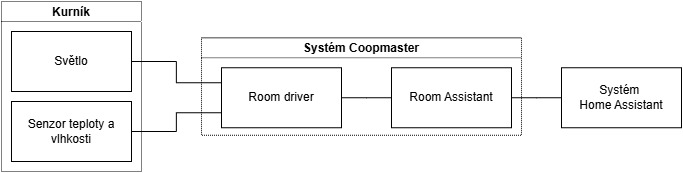
\includegraphics[width=\textwidth]{img/svetlo_teplo_vlhkost}
    \caption{Diagram ovládání světla a poskytování dat o teplotě a vlhkosti}
    \label{fig:svetlo_teplo_vlhkost}
\end{figure}

\subsection{Automatizace dvířek}
Hlavním z důvodů proč vznikl tento projekt, je zautomatizování raního otevírání a večerního zavírání dvířek v kurníku.
V této sekci si tedy zjednodušeně popíšeme princip, jak je v systému Coopmaster řešené automatické ovládání dvířek.
Graficky jsou závislosti mezi jednotlivými moduly vysvětleny v obrázku~\ref{fig:automatizace_dvirek}.\newline
Dvířka v našem systému jsou kontrolována pomocí modulu Řídící jednotka.
Room Driver zajišťuje pomocí USB sběrnice a HTTP protokolu komunikaci mezi Řídící jednotkou a Room Assistantem.
Room Assistant je jak již bylo zmíněno propojen se systémem Home Assistant pomocí MQTT protokolu.
Dále v této sekci potřebujeme získat data z kamerového systému konkrétně z kamery v kurníku.
Komunikaci s kamerovým systémem zajišťuje přes HTTP protokol modul Camera Driver.
Tento modul má vystavené RESTové api a poskytuje obrázky službám v systému Coopmaster.
O obrázky si zde říká služba Chicken Watch Guard, která za pomocí neuronové sítě konkrétně pak metody klasifikace počítá slepice v kurníku a výsledný počet posílá opět pomocí MQTT do Home Assistanta.
Chicken Watch Guard také předává co minutu do systému Home Assistant obrázek z kamery v kurníku.
Home Assistant pro tuto sekci zajišťuje indikaci stavu dvířek, ovládací tlačítka pro dvířka, vizualizaci počtu slepic v kurníku a zobrazuje fotografii pořízenou v kurníku.
Hlavním důvodem, proč je v projektu použit Home Assistant, je jeho funkcionaliza pro automatizaci různých operací.
Zde je toho právě využito pro automatizaci zavírání a otevírání dvířek.
Home Assistant je nakonfigurován tak, aby se od určitého časového okamžiku snažil zavřít dvířka pod podmínkou, že bude počet slepic, který identifikoval Chicken Watch Guard, stejný jako ten, jež jsme nastavili jako pevnou konstantu neboli aktuální počet slepic v kurníku.
\begin{figure}[h]
    \centering
    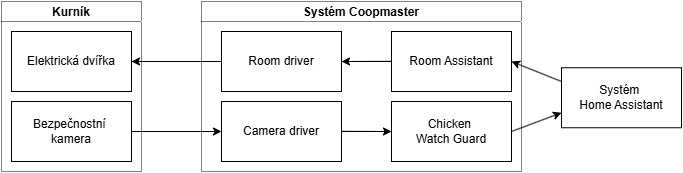
\includegraphics[width=\textwidth]{img/automatizace_dvirek}
    \caption{Diagram bezpečného zavření dvířek}
    \label{fig:automatizace_dvirek}
\end{figure}

\subsection{Detekce vetřelců}
Pro tento úkol bude třeba využít obrázků s kamery ve výběhu a umělé inteligence, která v obraze rozpozná určené vetřelce.
Princip komunikace je graficky vysvětlen v obrázku~\ref{fig:detekce_vetrelcu}.\newline
S kamerou ve výběhu komunikuje pomocí HTTP protokolu služba Camera Driver.
Z REST aplikačního rozhraní služby si stahuje obrázku služba Dog Alert.
Tato služba využívá neuronovou síť k detekci vetřelce v obraze.
Pokud detekováno nějaké nebezpečí, služba pomocí MQTT protokolu informuje systém Home Assistant a předá mu aktuální fotografii v níž byl vetřelec detekován jako důkaz.
Home Assistant je nastaven tak, že při přijetí takové zprávy, odešle uživateli do aplikace v mobilním telefonu oznámení, aby ho upozornil na detekci hrozby.
Dog Alarm dále pak každou minutu posílá do Home Assistanta aktuální snímek z kamery ve výběhu, aby měl uživatel stále přehled.
\begin{figure}[h]
    \centering
    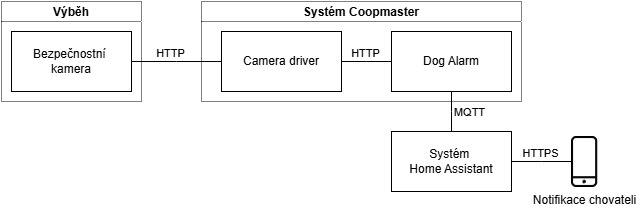
\includegraphics[width=\textwidth]{img/detekce_vetrelcu}
    \caption{Diagram detekce vetřelců}
    \label{fig:detekce_vetrelcu}
\end{figure}

\subsection{Vizualizace stavů hnízd}
Abychom splnili tento úkol, bude potřeba získat data z jednotlivých vah ve hnízdech.
Tato data pak dostat z do systému Coopmaster.
Coopmaster následně data vyhodnotí a výsledky předá k vizualizaci do systému Home Assistant.
Schémadické vyjádření principu pro vizualizaci stavů hnízd je znázorněno v obrázku~\ref{fig:vizualizace_stavu_hnizd}. \newline
Pro komunikaci s modulem Digitální váha je použita služba Scale Driver, která s jednotlivými váhami komunikuje přes USB sběrnici.
Data o váhách si ze Scale Driveru stahuje služba Nest Watcher.
Tato služba ukládá v daném intervalu data z každé váhy do databáze.
Služba po uplinutí časové konstanty analyzuje časovou řadu v databazi a vyhodnotí stav hnízda.
Detailní popis algoritmu v sekci o službě Nest Watcher (\ref{sec:nest-watcher}).
Po vyhodnocení stavů jsou data předávány pomocí MQTT protokolu do systému Home Assistant, který je díky na míru dělané komponentě zobrazí uživateli.
\begin{figure}[h]
    \centering
    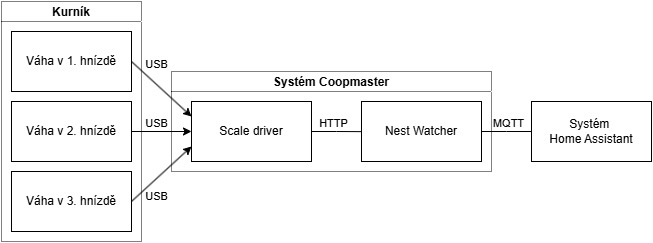
\includegraphics[width=\textwidth]{img/vizualizace_stavu_hnizd}
    \caption{Diagram vizualizace stavů hnízd}
    \label{fig:vizualizace_stavu_hnizd}
\end{figure}

\section{Zpřístupnění aplikace z internetu}\label{sec:zpristupneni-aplikace-z-internetu}
Aby systém mohl sloužit svému účelu musí být vzdáleně přístupný.
To znamená, že server, na kterém systém poběží, musí mít veřejnou ip adresu a v ideálním případě mít tuto adresu propojenou s doménovým názvem pro snadnější použití.
Tato problematika se dá řešit několika způsoby.\newline
Jeden ze způsobů je zařízení si přímo veřejné ip adresy pro svůj server.
Toto řešení je, technicky i teoreticky náročné, protože v případě, se kterým pracujeme my, běží server na lokální síti a veřejná ip adresa tedy není přímo pro náš server, ale celou síť.
To vytváří v určitých situacích vytváří velmi vážná bezpečnostní rizika, díky čemuž je tato metoda velice náročná na hardware a implementaci.
Navíc poskytování veřejné ip adresy je placená služba poskytovatel internetového připojení.\newline
Další způsob je nasazení části systému do některého z cloudových řešení jako je Microsoft Azure nebo Amazon AWS.
Tato metody by v podstatě vyhovovala našim požadavkům, ale pokud bychom se bavili o ceně, tak to rozhodně není levné řešení. \newline
Metoda, kterou využíváme v řešení my, je snadná, jednodužší na implementaci než zřizování veřejné ip adresy a levnější nez využití cloudové služba.
Tento způsob využívá takzvané tunely neboli šifrovaná spojení.
Funguje na principu, při němž se zařízení šifrovaně propojíte s veřejným serverem a tento server bude skrze sebe vystavovat službu, která běží na lokálním počítači například u nás doma.
Výhoda je, že vzdálený server disponuje kvalitním a odborně nastaveným firewalem, ktery zajistí dobrou ochranu našeho lokálního serveru.
Tuto službu poskytuje zdarma a bez omezení například společnost Cloudflare.
Tento způsob nejvíce odpovídá našim požadavkům, které byli cena a jednoduchost společně s rychlost nasazení.\newline
Poslední nutnostní, kterou ovšem je třeba zaplatit, je pronájem vlastního doménového jména.
Doménu si lze pronajmout u doménových registrátorů jako jsou GoDaddy, Hostinger nebo například Forpsi.
Ceny domén se odvíjí na základě jejího druhu a pohybují od 20 do 1500 korun za kus.
My v našem řešení využíváme službu Forpsi, protože s ní máme již předchozí zkušenost.\newline
Dále je tato část rozvedena v sekci~\ref{ch:nasazeni-do-kurniku}, kde je popsán konkrétní způsob nasazení do funkčního projektu.

\newpage